% !TeX spellcheck = cs_CZ
%{\tikzset{external/prefix={tikz/FYZI/}}
% \tikzset{external/figure name/.add={ch28_}{}}
%=========================== Kapitola: Elektromagnetické záření ===================================
\setchaptertoc
\chapter{Elektromagnetické záření}\label{fyz:IchapXXVIII}

  \section{Elektromagnetizmus}\label{fyz:IchapXXVIIIsecI}
    Nejdramatičtější okamžiky rozvoje fyziky jsou ty, v nichž dochází k velkým syntézám, kdy se 
    přijde na to, že jevy, které se předtím zdály být rozdílné, jsou jen různými stránkami stejné 
    věci. Historie fyziky je historií takových syntéz a základ úspěchu fyzikální vědy spočívá v 
    tom, že jsme schopni dělat syntézy.
   
    Snad nejdramatičtější okamžik v rozvoji fyziky v 19. století zažil \emph{J. C. Maxwell} jednoho 
    dne v roce 1860, když zkombinoval zákony elektřiny a magnetizmu se zákony chování světla. Jako 
    důsledek se podařilo zčásti rozuzlit vlastnosti světla - dávné a jemné substance, tak důležité 
    a tajemné, že při psaní knihy Genesis jí byl vyhrazen zvláštní akt stvoření. Když Maxwell 
    dokončil svůj objev, mohl říci: „Budiž elektřina a magnetizmus, a je světlo!“
    
    Tento kulminační okamžik se dlouho připravoval v postupném objevování a odhalování zákonů 
    elektřiny a magnetizmu. Stručně to bylo asi takto: Postupným objevováním vlastností elektřiny a 
    magnetizmu, elektrických přitažlivých a odpudivých sil a magnetických sil se ukázalo, že 
    ačkoliv jsou všechny tyto síly dost složité, všechny se zmenšují jako převrácená hodnota druhé 
    mocniny vzdálenosti. Příkladem může být známý Coulombův zákon elektrostatických sil mezi 
    nehybnými náboji. V důsledku toho při dostatečně velkých vzdálenostech jeden systém nábojů jen 
    velmi málo ovlivní druhý systém nábojů. Když se Maxwell pokoušel shrnout všechny rovnice nebo 
    zákony, jež byly do té doby objeveny, všiml si, že jsou vzájemně nekonzistentní a k tomu, aby 
    se celý systém stal konzistentním, musel ke svým rovnicím přidat další člen. S tímto novým 
    členem dostal překvapující předpověď, že část elektrického a magnetického pole by se měla 
    zmenšovat mnohem pomaleji v závislosti na vzdálenosti než převrácená hodnota její druhé 
    mocniny, a to jako převrácená hodnota první mocniny vzdálenosti! Tak si uvědomil, že elektrické 
    proudy na jednom místě mohou ovlivnit jiné velmi vzdálené náboje a předpověděl nám dnes dobře 
    známé základní jevy - přenos rádiových vln, radar apod.
    
    Zdá se, že je to zázrak, když někoho, kdo mluví v Evropě, můžeme slyšet jen pomocí pouhých 
    elektrických vlivů tisíce kilometrů daleko v Los Angeles. Jak je to možné? Je to tím, že pole 
    se nemění s převrácenou hodnotou druhé mocniny, ale jen s převrácenou hodnotou první mocniny 
    vzdálenosti. Nakonec se zjistilo, že samotné světlo jsou elektrické a magnetické vlivy šířící 
    se na ohromné vzdálenosti, vytvořené téměř neuvěřitelně rychlými oscilacemi elektronů v 
    atomech. Všechny tyto jevy zahrnujeme pod název záření, přesněji elektromagnetické záření, 
    neboť existuje ještě jeden nebo dva další druhy záření. Slovo záření téměř vždy znamená 
    elektromagnetické záření.
    
    A tak je celý vesmír propojen. Atomové pohyby ve vzdálených hvězdách mají na tak velkou 
    vzdálenost dostatečný vliv na to, aby uvedly do pohybu elektrony v našem oku - a tak víme o 
    tom, že jsou hvězdy. Kdyby tento zákon neplatil, byli bychom, pokud jde o vnější svět, v 
    naprosté temnotě! Elektrické vlnobití v galaxii vzdálené mnoho miliard světelných let, může 
    ještě významně a pozorovatelně ovlivnit proudy ve velkém „talíři“ před naším radioteleskopem. 
    Proto vidíme hvězdy a galaxie. 
    
    Tento pozoruhodný jev bude předmětem naší diskuze v této kapitole. Na začátku tohoto kurzu 
    fyziky jsme si načrtli hrubý obraz světa, ale nyní jsme lépe připraveni na to, abychom 
    pochopili některé jeho stránky. A tak si projdeme některé jeho části podrobněji. Začneme 
    popisem postavení fyziky na konci 19. století. Vše, co bylo tehdy známo o fyzikálních zákonech, 
    lze shrnout takto: 
    
    Byly zde nejprve zákony sil; jedním z nich byl gravitační zákon, který jsme si napsali 
    několikrát. Síla působící na objekt o hmotnosti \(m\), způsobená jiným objektem \(M\), je dána 
    vztahem
    \begin{equation}\label{fyz:eq296}
      \vec{F} = \kappa\dfrac{m\cdot M}{r^2}\vec{r}_0,
    \end{equation}
    
    kde \(\vec{r}_0\) je jednotkový vektor ve směru od \(m\) k \(M\) a \(r\) je vzdálenost mezi 
    nimi.
    
    Dále tady byly zákony elektřiny a magnetizmu, jak byly známy na konci 19. století. Jsou to tyto 
    zákony: Elektrické síly působící na náboj \(q\) lze popsat pomocí dvou polí označených jako 
    \(\vec{E}\) a \(\vec{B}\) a rychlosti \(\vec{v}\) náboje \(q\) podle rovnice
    \begin{equation}\label{fyz:eq297}
      \vec{F} = q (\vec{E} + \vec{v}\times\vec{B}). 
    \end{equation}
    Pro úplnost musíme dodat, jak jsou vyjádřena \(\vec{E}\) a \(\vec{B}\) za daných okolností. Za 
    přítomnosti více nábojů jsou \(\vec{E}\) a \(\vec{B}\) rovny součtu příspěvků od jednotlivých 
    nábojů. Takže, umíme-li najít \(\vec{E}\) a \(\vec{B}\) způsobené jedním nábojem, potřebujeme k 
    určení celkového \(\vec{E}\) a \(\vec{B}\) pouze sečíst účinky všech nábojů ve vesmíru! To je 
    princip \textbf{superpozice}.
    
    Jaký je vztah pro elektrické a magnetické pole vytvořené jedním nábojem? Ukazuje se, že je to 
    velmi komplikovaný vztah a k jeho pochopení je třeba hodně studovat a přemýšlet. O to tu ale 
    nejde. Nyní si uvedeme tento zákon, jen tak, abychom na čtenáře zapůsobili krásou přírody, tj. 
    abychom ukázali, že je možné shrnout všechny základní poznatky na jednu stranu textu a to 
    pomocí notace, s níž je už teď obeznámen. Zákon určující pole jednotlivého náboje je, pokud 
    víme, úplný a přesný (kromě kvantové mechaniky), vypadá však dost komplikovaně. Nebudeme 
    studovat jeho jednotlivé části, jen si ho napíšeme, abychom ukázali, že jej lze napsat a 
    abychom už napřed viděli, jak vypadá. Vlastně, nejlepší způsob zápisu zákonů elektrického a 
    magnetického pole není ten, který nyní použijeme, ale zahrnuje tzv. \emph{rovnice pole}, jimiž 
    se budeme zabývat později. Matematická symbolika těchto rovnic je odlišná a nová. Proto si 
    tento zákon zapíšeme ve formě, jež sice není vhodná pro výpočty, ale pomocí symboliky, kterou 
    známe. 
    
    Intenzita elektrického pole \(\vec{E}\) je dána vztahem
    \begin{equation}\label{fyz:eq298}
      \vec{E} = -\frac{q}{4\pi\varepsilon_0}\left[
                 \frac{\vec{r}_0}{r'^2} + 
                 \frac{r'}{c}\der{ }{t}\left(\frac{\vec{r}_0}{r'^2}\right) +
                 \frac{1}{c^2}\dder{ }{t}\vec{r}_0
                 \right].
    \end{equation}
    Co nám říkají jednotlivé členy? Vezměme si první výraz
    \begin{equation*}
      \vec{E} = -\frac{q}{4\pi\varepsilon_0}\frac{\vec{r}_0}{r'^2}. 
    \end{equation*}
    což je, samozřejmě, \emph{Coulombův zákon}, který už známe. Zde \(q\) je náboj vytvářející 
    pole, \(\vec{r}_0\) je \emph{jednotkový vektor} ve směru od bodu \(P\), v němž měříme pole, 
    \(r\) je \emph{vzdálenost} z \(P\) do \(q\). Coulombův zákon však není správný. Objevy 19. 
    století ukázaly, že působení se nemohou šířit rychleji, než je určitá základní rychlost \(c\), 
    kterou nyní nazýváme \emph{rychlost světla}. Není správné tvrdit, že první člen je Coulombův 
    zákon a nejen proto, že nemůžeme vědět, kde se nyní náboj nachází a jak je vzdálený, ale také 
    proto, že jediné, co může ovlivnit pole na daném místě v daném okamžiku je chování nábojů v 
    minulosti. V jak dávné minulosti? Toto zpoždění času (\emph{retardace času}) je rovno času 
    potřebnému k překonání vzdálenosti od náboje do bodu \(P\) rychlostí \(c\). Zpoždění je rovno 
    \(r'/c\). 
    
    Abychom vzali v úvahu zpoždění času, přidáváme k \(r\) malou čárku, což označuje vzdálenost, 
    jež existovala mezi \(P\) a \(q\) v čase, kdy informace, jež právě dorazila k \(P\) opustila 
    \(q\). Na chvíli předpokládejme, že náboj svítil a že toto světlo mohlo dojít k \(P\) pouze 
    rychlostí \(c\). Pak bychom při pohledu na \(q\) neviděli, kde se nyní nachází, ale kde byl 
    před nějakou dobou. Veličina, jež v našem vzorci vystupuje, je zdánlivý směr \(\vartheta_{r'}\) 
    - směr, kde byl náboj předtím - tj. \emph{retardovaný směr} a \(r'\) je \emph{retardovaná 
    vzdálenost}. To by již bylo možné pochopit, ale ani to není správné. Celá věc je mnohem 
    komplikovanější. 
    
    Ve vzorci je více členů. Další člen jakoby svědčilo tom, že příroda bere v úvahu retardační 
    efekt, velmi hrubě řečeno. Ukazuje na to, že bychom měli vypočítat zpožděné coulombovské pole a 
    přičíst k němu opravu rovnou rychlosti změny pole násobené zpožděním času. Zdá se, že příroda 
    se pokouší odhadnout, čemu se v současnosti bude pole rovnat, a to pomocí rychlosti změny 
    vynásobené časovým zpožděním. Stále však nejsme na konci. Je zde ještě třetí člen - druhá 
    derivace podle \(t\) jednotkového vektoru ve směru náboje. Vzorec je nyní hotov, a to je vše, 
    co se týká intenzity elektrického pole libovolně se pohybujícího 
    náboje\footnote{Nerelativistickými rychlostmi.}.
    
    Magnetické pole je dáno vztahem
    \begin{equation}\label{fyz:eq299}
      \vec{B} = -\vec{r}_0\times\frac{\vec{E}}{c}
    \end{equation}
    Tyto vzorce jsme si uvedli proto, abychom ukázali krásu přírody nebo určitým způsobem, sílu 
    matematiky. Nečiníme si nárok na pochopení, proč je možné tak mnoho napsat na tak malém 
    prostoru, ale vztahy (\ref{fyz:eq298}) a (\ref{fyz:eq299}) obsahují podstatu elektrických 
    generátorů, světla a všech jevů elektřiny a magnetizmu. Samozřejmě, aby věc byla úplná, musíme 
    také něco vědět o chování materiálů - o vlastnostech hmoty, jež nejsou pomocí (\ref{fyz:eq298}) 
    přiměřeně popsány.
    
    Abychom dokončili náš popis světa 19. století, musíme se zmínit ještě o jedné velké syntéze, 
    kníž v tomto století došlo a jež se také týkala do značné míry Maxwella, a to syntézy tepelných 
    jevů a mechaniky. Tento předmět budeme brzy studovat.
   
    Ve 20. století bylo dále zjištěno, že všechny Newtonovy dynamické zákony jsou chybné a k jejich 
    opravě bylo třeba zavést kvantovou mechaniku. Newtony zákony platí přibližně pro jevy a věci, 
    jež mají dostatečně velké rozměry. Zákony kvantové mechaniky byly zkombinovány se zákony 
    elektřiny teprve nedávno a tak vznikla řada zákonů nazvaných \emph{kvantová elektrodynamika} 
    Navíc bylo objeveno mnoho nových jevů, prvním byla radioaktivita, objevená Becquerelem r. 1898 
    těsně na konci 19. století. Studium radioaktivity přineslo poznatky o jádrech a o nových 
    druzích sil, jež nejsou ani gravitační ani elektrické, ale působí mezi novými částicemi s 
    různými interakcemi, a tyto jevy nebyly ještě dostatečně prozkoumány.
    
    Pro ty puntičkáře, kteří toho vědí víc (profesorům, kteří snad budou číst tento text), bychom 
    měli dodat, že označujeme-li (\ref{fyz:eq298}) za úplné vyjádření poznatků elektrodynamiky, 
    nejsme zcela přesní. Existoval problém, jež nebyl koncem 19. století zcela vyřešen. Pokusíme-li 
    se vypočítat pole působící na náboj od všech nábojů, včetně náboje samotného, dostaneme se do 
    těžkostí například při určování vzdálenosti náboje od sebe samého a při dělení touto veličinou 
    rovnou nule. Dodnes není vyřešen problém zacházení s tou částí pole, jež je vytvořena samotným 
    nábojem, na nějž chceme, aby pole působilo. Takže to necháme stranou; neznáme ještě úplné 
    řešení této hádanky, proto se jí budeme vyhýbat, jak jen to bude možné.
    
  \section{Záření}\label{fyz:IchapXXVIIIsecII}
    Udělali jsme souhrn obrazu světa. Nyní ho použijeme při probírání jevu nazvaného záření. 
    Abychom mohli tento jev zkoumat, musíme vybrat z rovnice (\ref{fyz:eq298}) tu část, která se 
    mění nepřímo úměrně vzdálenosti a ne druhé mocnině vzdálenosti. Ukázalo se, že tato část 
    rovnice má tak jednoduchý tvar, že jsme oprávněni studovat optiku a elektrodynamiku 
    elementárním způsobem na základě tohoto „zákona“ pro elektrické pole vytvořené pohybujícím se 
    vzdáleným elektrickým nábojem. Dočasně si ho vezmeme jako daný zákon.
   
    První z členů, jež vystupují v (\ref{fyz:eq298}), závisí celkem jasně na převrácené hodnotě 
    druhé mocniny vzdálenosti a druhý je jen korekcí zpoždění, takže lze snadno ukázat, že oba se 
    mění s převrácenou hodnotou druhé mocniny vzdálenosti. Všechny jevy, o něž se zajímáme, 
    pocházejí z třetího členu, který není koneckonců příliš komplikovaný. Říká toto: Podívej se 
    směrem k náboji a všimni si směru jednotkového vektoru (jeho konec můžeme promítnout na povrch 
    jednotkové koule). Při pohybu náboje jednotkový vektor mění směr a zrychlení tohoto 
    \emph{jednotkového vektoru je to, co hledáme}. To je vše. Takže:
    \begin{equation}\label{fyz:eq300}
      \vec{E} = -\frac{q}{4\pi\varepsilon_0c^2}\dder{\vec{r}_0}{t}.
    \end{equation}
    vyjadřuje zákon záření, neboť když se dostatečně vzdálíme, je to jediný důležitý člen, který se 
    mění nepřímo úměrně vzdálenosti. (Ty části, jež závisí na druhé mocnině vzdálenosti, se natolik 
    zmenšily, že se o ně nezajímáme.) 
    
    Nyní můžeme vztah (\ref{fyz:eq300}) studovat trochu podrobněji, abychom zjistili, co znamená. 
    Předpokládejme, že náboj se nějakým způsobem pohybuje a m yho pozorujeme z určité vzdálenosti. 
    Na chvíli si představme, že náboj „svítí“ (přestože je to právě světlo, co chceme vysvětlit). 
    Představme si ho jako malou bílou tečku, takže uvidíme, jak se tato tečka pohybuje kolem 
    dokola. Nevidíme však přesně jak se pohybuje právě ted, a to pro zpoždění, o němž jsme mluvili 
    Záleží na tom, jak se pohybovala dříve. Jednotkový vektor \(\vec{r}_0\) míří směrem zdánlivé 
    polohy náboje. Pohybuje-li se \(\vec{r}_0\) po mírné křivce, jeho zrychlení má dvě složky. 
    Jednou z nich je příčná složka, neboť konec \(\vec{r}_0\) se pohybuje nahoru a dolů a druhou je 
    podélná složka, neboť konec \(\vec{r}_0\) zůstává na kulové ploše. Snadno lze ukázat, že druhá 
    složka je mnohem menší a že se mění převráceně s druhou mocninou \(\vec{r}\), je-li \(\vec{r}\) 
    velmi velké. Snadno si to uvědomíme, když si představíme, že daný zdroj vzdalujeme více a více. 
    Potom se chvění \(\vec{r}_0\) zdá být stále menší a menší úměrně převrácené hodnotě 
    vzdálenosti, ale podélná složka zrychlení se mění mnohem rychleji než převrácená hodnota 
    vzdálenosti. Pro praktické účely nám stačí udělat projekci pohybu na rovinu v jednotkové 
    vzdálenosti. Nalézáme toto pravidlo: Představme si, že se díváme na pohybující se náboj a vše, 
    co vidíme je zpožděné - jako malíř, který se pokouší malovat scénu na plátno v jednotkové 
    vzdálenosti. Samozřejmě, že skutečný malíř nebere v úvahu, že se světlo šíří určitou rychlostí, 
    ale maluje svět, jak ho vidí. Chceme vidět, jak vypadá jeho obraz. Vidíme tečku, znázorňující 
    náboj, pohybující se po obraze. Zrychlení tohoto bodu je úměrné intenzitě elektrického pole. To 
    je vše, co potřebujeme.
    
    Rovnice (\ref{fyz:eq300}) je tedy úplným a správným vztahem pro záření; dokonce obsahuje 
    všechny relativistické efekty. Často ji však chceme aplikovat na ještě jednodušší situaci, v 
    níž se pohybují náboje pouze na krátké vzdálenosti poměrně malou rychlostí. Pohybují-li se 
    pomalu, nedostanou se příliš daleko, takže časové zpoždění je prakticky konstantní. Náš zákon 
    je potom ještě jednodušší, neboť zpoždění je fixováno. Představujme si proto, že náboj koná 
    velmi malý pohyb v efektivně neměnné vzdálenosti. Zpoždění při vzdálenosti \(r\) je ](r/c). 
    Pravidlo je pak takové: vykonává-li nabitý předmět malý pohyb do strany na vzdálenost \(x(t)\), 
    potom úhel, o nějž se posune jednotkový vektor \(\vec{r}_0\), je roven \(x/r\), a protože \(r\) 
    je prakticky konstantní, je \(x\)-ová složka \(\dder{\vec{r}_0}{t}\) rovna prostě zrychlení 
    \(x\) v nějakém dřívějším čase, takže nakonec dostáváme zákon, který jsme chtěli
    \begin{equation}\label{fyz:eq301}
      E_x(t) = -\frac{q}{4\pi\varepsilon_0c^2r}a_x\left(t-\frac{r}{c}\right).
    \end{equation}
    Důležitá je jen složka \(a_x\) kolmá na směr pohledu. Podívejme se, proč tomu tak je. Je jasné, 
    že když se náboj pohybuje ve směru k nám sem a tam, jednotkový vektor ve směru náboje se
    vůbec nemění a nezrychluje. Takže důležitý je pouze příčný pohyb, pouze zrychlení, které vidíme 
    promítnuté na stínítko.
    
  \section{Dipólový zářič}\label{fyz:IchapXXVIIIsecIII}
    Za náš základní „zákon“ pro elektromagnetické záření budeme považovat vztah (\ref{fyz:eq301}), 
    o němž budeme předpokládat, že je přesný, tj. že elektrické pole vytvořené zrychleným 
    nerelativistickým pohybem náboje lze popsat na velmi velkých vzdálenostech \(r\) tímto vztahem. 
    Elektrické pole se mění nepřímo úměrně \(r\) a je úměrné zrychlení náboje promítnutému do 
    „roviny pohledu“, přičemž toto zrychlení není dnešním zrychlením, ale zrychlením, jímž se náboj 
    pohyboval v dřívějším čase a čas zpoždění je roven \(r/c\). Ve zbývající části této kapitoly si 
    prodiskutujeme tento zákon, abychom mu lépe fyzikálně rozuměli, neboť ho chceme použít při 
    výkladu všech jevů týkajících se šíření světla a rádiových vln jako jsou odraz, lom, 
    interference, ohyb a rozptyl. Je to ústřední zákon a je to vše, co potřebujeme. Celý zbytek 
    rovnice (\ref{fyz:eq298}) jsme si uvedli jen pro celkový rámec, abychom pochopili, kam 
    (\ref{fyz:eq301}) zapadá a odkud pochází. 

    \begin{figure}[ht!] %\ref{fyz:fig0228}
      \centering
      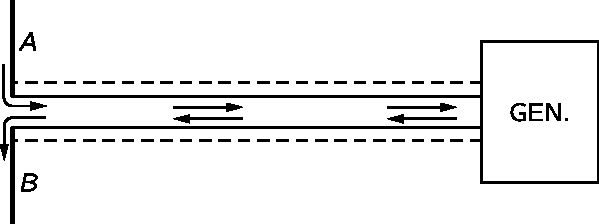
\includegraphics[width=0.5\linewidth]{fyz_fig0228.pdf}
      \caption{Generátor vysokofrekvenčního signálu pohybuje náboji ve dvou drátech nahoru a dolů
               (\cite[s.~375]{Feynman01})}
      \label{fyz:fig0228}
    \end{figure}
    
    O vztahu (\ref{fyz:eq298}) budeme diskutovat později. Zatím ho přijmeme za správný a to nejen 
    teoreticky. K ilustraci tohoto zákona bychom mohli navrhnout řadu experimentů. Potřebujeme k 
    tomu zrychlující se náboj. Měl by to být jeden náboj, ale pokud můžeme dosáhnout současného 
    pohybu velkého množství nábojů, nic se nestane, neboť víme, že pole bude dáno součtem účinků 
    jednotlivých nábojů - prostě je sečteme. Jako příklad si vezmeme dva kusy drátu spojené s 
    generátorem, jak je znázorněno na obr. \ref{fyz:fig0228}. Generátor vytváří rozdíl potenciálů 
    nebo pole, které v jednom okamžiku odtahuje elektrony pryč z kousku \(A\) a odvádí je do kousku 
    \(B\) a potom o infinitezimální čas později se změní jeho účinek a elektrony se pohybují zpět 
    do \(A\)! V těchto drátech jsou v jednom okamžiku náboje urychlovány, dejme tomu směrem nahoru 
    a v dalším okamžiku jsou v drátech \(A\) i \(B\) urychlovány směrem dolů. Skutečnost, že 
    potřebujeme dva dráty a generátor, souvisí s tím, že tak se to provádí v praxi. Konečný 
    výsledek je takový, že náboj se urychluje nahoru a dolů, jakoby \(A\) a \(B\) tvořily jediný 
    drát. Drát, který je velmi krátký v porovnání se vzdáleností, kterou světlo projde za jednu 
    periodu, se nazývá \textbf{elektrický dipólový oscilátor}. Tím jsou tedy splněny podmínky, 
    abychom mohli použít náš zákon, který říká, že takový náboj vytváří elektrické pole. Ještě 
    potřebujeme přístroj na detekci tohoto elektrického pole. Přístroj, který k tomu použijeme, je 
    stejný - je to pár drátů jako \(A\) a \(B\) Působí-li na takové zařízení elektrické pole, 
    vyvolá sílu, jež bude v obou drátech pohybovat elektrony nahoru nebo dolů. Takový signál lze 
    detekovat pomocí usměrňovače zapojeného mezi \(A\) a \(B\) a pomocí drátku se tato informace 
    přenáší na zesilovač, kde se natolik zesílí, že můžeme slyšet tón o zvukové frekvenci, jímž je 
    radiofrekvence modulována. Pocítí-li tento snímač elektrické pole, začne z reproduktoru znít 
    silný zvuk a není-li zde elektrické pole, zvuk nevznikne.

    Protože v místnosti, kde měříme vlny, jsou umístěny i jiné objekty, naše elektrické pole 
    rozkmitá elektrony i v těchto objektech. Elektrické pole způsobí, že tyto další náboje budou 
    kmitat a tím budou také působit na náš snímač. Proto, aby experiment byl úspěšný, musí obě 
    zařízení být blízko sebe, aby vlivy od stěna nás samotných - odražené vlny - byly relativně 
    malé. Proto se ukáže, že zkoumaný jev není v přesném dokonalém souladu srovnicí 
    ((\ref{fyz:eq301})), ale soulad bude dostatečně dobrý, abychom mohli ocenit platnost tohoto 
    zákona.
    
    \begin{figure}[ht!] %\ref{fyz:fig0229}
      \centering
      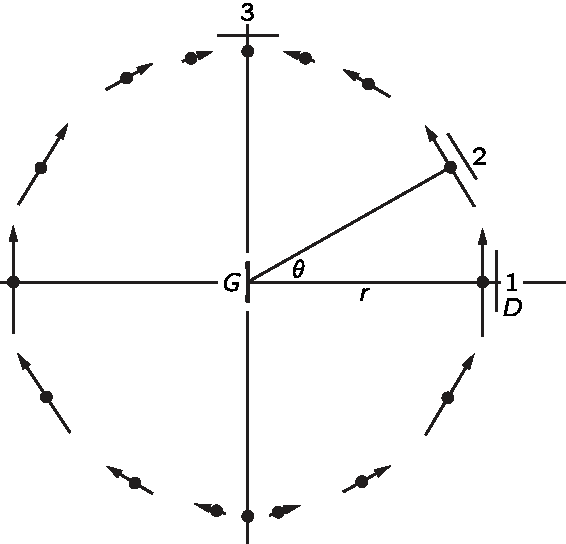
\includegraphics[width=0.5\linewidth]{fyz_fig0229.pdf}
      \caption{Okamžité elektrické pole na kulové ploše, která má ve středu lineárně oscilující 
               náboj (\cite[s.~376]{Feynman01})}
      \label{fyz:fig0229}
    \end{figure}

    Při zapnutí generátoru \(G\) slyšíme zvukový signál. Je-li detektor \(D\) rovnoběžný s \(G\), v 
    bodě \(1\) zaznamená silné elektrické pole (obr. \ref{fyz:fig0229}). Pod jakýmkoliv azimutálním 
    úhlem vzhledem k ose \(G\) zjistíme stejné pole, neboť \(G\) nemá směrové účinky. Na druhé 
    straně, pro detektor v poloze \(3\) je pole nulové. To je zcela v pořádku, neboť náš vztah 
    říká, že pole bude úměrné průmětu zrychlení náboje kolmému ke směru pohledu. Proto, když se 
    díváme dolů na \(G\), náboj se pohybuje dopředu a dozadu od \(D\), takže nevzniká žádný efekt. 
    Tím je ověřeno první pravidlo: Když se náboj pohybuje ve směru přímo k nám, nevyvolává žádný 
    účinek. Za druhé, náš vztah říká, že elektrické pole má být v rovině, v níž leží \(G\) a \(r\), 
    kolmé na \(r\); takže, umístíme-li \(D\) do bodu \(1\), ale otočíme ho o \ang{90}, nedostaneme 
    žádný signál. Tak zjišťujeme, že elektrické pole je skutečně vertikální a ne horizontální. 
    Přemístíme-li \(D\) do nějaké střední polohy \(2\), zjistíme, že nejsilnější signál je tehdy, 
    když \(D\) je orientováno jako na obr. \ref{fyz:fig0229}. I když \(G\) je vertikální,
    nevyvolává pole, které by s ním bylo prostě rovnoběžné - to, co se projevuje, je kolmý průmět 
    zrychlení do směru pohledu. Právě proto je v bodě \(2\) signál slabší než v bodě \(1\).
    
  \section{Interference}\label{fyz:IchapXXVIIIsecIV}
    Dále si můžeme ověřit, co se stane, máme-li vedle sebe dva zdroje vzdálené několik centimetrů 
    (obr. \ref{fyz:fig0230}). Zákon říká, že účinky dvou zdrojů se mají sčítat v bodě \(1\), jsou-li 
    oba zdroje napájeny ze stejného generátoru a jsou-li pohyby nábojů nahoru a dolů v obou 
    současné, takže celkové elektrické pole je rovno součtu obou polí a je dvakrát silnější než 
    předtím.
    
    \begin{figure}[ht!] %\ref{fyz:fig0230}
      \centering
      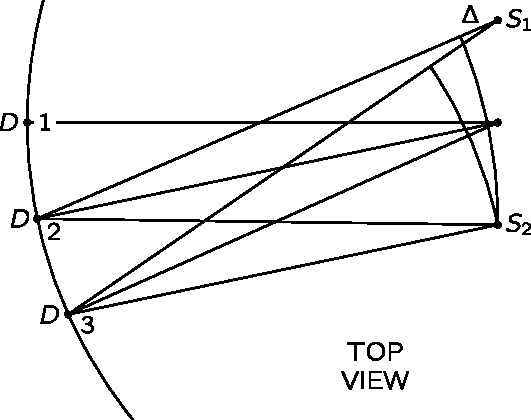
\includegraphics[width=0.5\linewidth]{fyz_fig0230.pdf}
      \caption{Znázornění interference zdrojů
               (\cite[s.~377]{Feynman01})}
      \label{fyz:fig0230}
    \end{figure}
    
    Nyní vzniká zajímavá možnost. Předpokládejme, že náboje v \(S_1\) a \(S_2\) se zrychlují směrem 
    nahoru a dolů, ale že \(S_2\), se zpožďuje za \(S_1\), takže jsou fázově posunuty o \ang{180}. 
    Pole vytvořené zdrojem \(S_1\) pak bude mít jeden směr a pole vytvořené zdrojem \(S_2\) opačný 
    směr, a proto bychom v bodě \(1\) neměli naměřit žádné účinky. Fázi oscilací lze snadno měnit 
    pomocí přívodu, jenž přivádí signál na \(S_2\). Změnou délky tohoto přívodu změníme dobu, 
    kterou potřebuje signál, aby se dostal na \(S_2\), a tím změníme fázi oscilací. Nastavením této 
    délky můžeme skutečně najít takové místo, kde přesto, že \(S_1\) a \(S_2\) pracují, není žádný 
    signál. To, že oba zdroje pracují, lze snadno zjistit, neboť, když odpojíme jeden z nich, druhý 
    můžeme slyšet. Takže oba zdroje mohou mít nulové účinky, je-li všechno správně nastaveno.
    
    Velmi zajímavé je ukázat, že skládání dvou polí je skutečně vektorovým součtem. Přesvědčili 
    jsme se o tom již při pohybu vertikálním, ale ověřme si dva nerovnoběžné směry. Nejdříve 
    vrátíme \(S_1\) a \(S_2\) do původní situace, tj. aby byly ve fázi, takže oba systémy se 
    pohybují současně. Nyní ale otočíme \(S_1\) o \ang{90}, jak je znázorněno na obr. 
    \ref{fyz:fig0231}. V bodě \(1\) bychom měli mít součet dvou účinků, z nichž jeden je vertikální 
    a druhý horizontální. Elektrické pole je vektorovým součtem těchto dvou signálů, jež jsou ve 
    fázi - oba jsou současně silné a současně nulové. Celkové pole by mělo tvořit signál \(R\) pod 
    úhlem \ang{45}. Pootočíme-li \(D\) tak, abychom dostali maximální signál, mělo by to být v úhlu 
    kolem \ang{45}, a ne vertikálně. Pootočíme-li \(D\) do pravých úhlů s tímto směrem, měli bychom 
    dostat nulový signál, což lze snadno změřit. Skutečně, právě takové chování zjistíme!
    
    \begin{figure}[ht!] %\ref{fyz:fig0231}
      \centering
      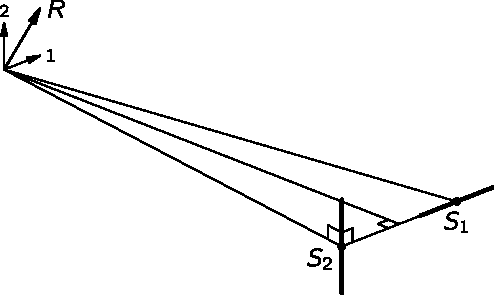
\includegraphics[width=0.5\linewidth]{fyz_fig0231.pdf}
      \caption{Znázornění vektorového skládání polí
               (\cite[s.~377]{Feynman01})}
      \label{fyz:fig0231}
    \end{figure}
    
    Jak se nyní projeví retardace? Jak můžeme ukázat, že signál je retardovaný? Pomocí složitého 
    zařízení bychom mohli měřit čas, za který přijde signál, ale existuje ještě jiný velmi 
    jednoduchý způsob. Vraťme s k obr. \ref{fyz:fig0230} a předpokládejme, že \(S_1\) a \(S_2\) jsou 
    ve fázi. Oba zdroje kmitají současně a v bodě \(1\) vytvářejí stejné elektrické pole. 
    Předpokládejme však, že přejdeme do určitého bodu \(2\), který je blíž k \(S_2\) a dál od 
    \(S_1\). Pak podle principu, že zrychlení mají být retardována o čas \(r/c\), pokud nejsou tato 
    zpoždění stejná, signály už nebudou ve fázi. Proto by mělo být možné najít takovou polohu, pro 
    niž se vzdálenosti \(D\) od \(S_1\) a od \(S_2\) liší o nějakou hodnotu \(\Delta\) takovou, že 
    výsledný signál je nulový. Vzdálenost \(\Delta\) má být tedy rovna vzdálenosti, kterou světlo 
    proletí za poloviční periodu oscilace generátoru. Můžeme se posunout ještě dál a najít bod, v 
    němž tento rozdíl odpovídá celé periodě, tj. signál z první antény dosáhne bodu \(3\) s časovým 
    zpožděním, jež je větší než časové zpoždění od druhé antény, a to právě o dobu, za niž     
    proběhne jeden kmit elektrického proudu. Proto jsou obě elektrická pole vytvořená v bodě \(3\) 
    znovu ve fázi a signál je opět silný.
    
    Tím končí naše diskuze o experimentálním ověření některých důležitých stránek rovnice 
    (\ref{fyz:eq300}). Samozřejmě, neověřili jsme si závislost \(1/r\) intenzity elektrického pole 
    nebo skutečnost, že společně s elektrickým polem se šíří i magnetické pole. To by si vyžadovalo 
    použití dost komplikovaných zařízení a v tomto bodě by nám to sotva pomohlo k lepšímu pochopení 
    věci. Ale ověřili jsme si ty vlastnosti jež jsou nejdůležitější pro naše další aplikace a ke 
    studiu dalších vlastností elektromagnetických vln se ještě vrátíme.
    
  \section{Příklady a cvičení}\label{fyz:IchapXXVIIIsecV}

%} %tikzset
%---------------------------------------------------------------------------------------------------